\documentclass[12pt]{article}
\usepackage{titlesec}
\usepackage{graphicx}
\usepackage{floatrow}

\titlelabel{\thetitle.\quad}
\titleformat*{\section}{\bf\normalsize}
\titleformat*{\subsection}{\bf\normalsize}

\begin{document}

\begin{flushright}
PBNC2014-218
\end{flushright}

\begin{center}
\textbf{COMBINED FIRE MODEL UNCERTAINTY AND INPUT PARAMETER UNCERTAINTY ANALYSIS FOR NUCLEAR POWER PLANT SCENARIOS}
% \textbf{A MONTE CARLO ANALYSIS OF THE EFFECT OF FIRE SEVERITY ON NUCLEAR SAFETY STRUCTURES, SYSTEMS, AND COMPONENTS}
\end{center}

\begin{center}
M. Clouthier\textsuperscript{1}, K. Overholt\textsuperscript{2}\\

\textsuperscript{1}Clouthier Risk Engineering, Nova Scotia, Canada\\
\textsuperscript{2}National Institute of Standards and Technology, Gaithersburg, MD, USA
\end{center}

\begin{center}
\textbf{Abstract}
\end{center}

Quantitative fire risk analysis is used in conducting safety assessments at nuclear facilities to evaluate the potential consequences of postulated fire scenarios.

In fire modelling applications, the key phenomena that influence the predicted figure of merit (i.e., the specific objective of the analysis) are known; however, in some cases the existing state of knowledge and the adequacy of existing modelling tools to predict a given phenomenon is in need of improvement. It is therefore necessary to consider relevant uncertainties in a rational quantitative manner.

In this paper, a Monte Carlo analysis is applied to a fire scenario involving potential damage to nuclear safety structures, systems, and components. The effect of deterministic peak heat release rate and fire growth on the predicted hot gas layer is studied. The results of the case study are presented to demonstrate an improved method to develop a design basis fire.

\section{Introduction}
\label{sec:introduction}

Model bias and uncertainty has been quantified in NRC NUREG-1824~\cite{NUREG_1824_Sup_1}. Each model input has some amount of uncertainty associated with it. These are addressed separately in NRC NUREG-1934~\cite{NUREG_1934}. In this paper, we demonstrate the calculation of three cases: 1) only considering model bias and uncertainty, 2) only considering input parameter uncertainty, and 3) combined analysis of model bias/uncertainty and input parameter uncertainty.

\section{Previous work}
\label{sec:previous_work}

Previous work on Monte Carlo analyses.


\section{Fire model scenario setup}
\label{sec:fire_model_scenario_setup}

Appendix B from NRC NUREG-1934~\cite{NUREG_1934} was selected. The Consolidation Model of Fire Growth and Smoke Transport (CFAST)~\cite{CFAST_Users_Guide_6} zone model was used. The compartment has dimensions of 26.5~m by 18.5~m by 6.1~m. The ambient temperature was specified as 20~$^\circ$C. The simulation time is 1~h. The wall and ceiling materials were specified as concrete with a thermal conductivity of XX~W/m-K, density of XX~kg/m$^3$, and specific heat of XX~J/g-K.


\section{Uncertainty analysis}
\label{sec:uncertainty_analysis}

Input: nominal HRR of 500~kW.
Output: threshold HGL temperature of 100~$^\circ$C.

\subsection{Case 1: Model bias and uncertainty}

This case accounts for model bias and uncertainty.

A HRR of 500~kW was selected as the input fire size.

The model bias $\delta$ for forced ventilation for the CFAST zone model is 1.15, and the model relative standard deviation $\widetilde\sigma_M$ is 0.20.

The results of Case 1 are shown in Fig.~\ref{fig:case_1_output_distributions}

\begin{figure}[!ht]
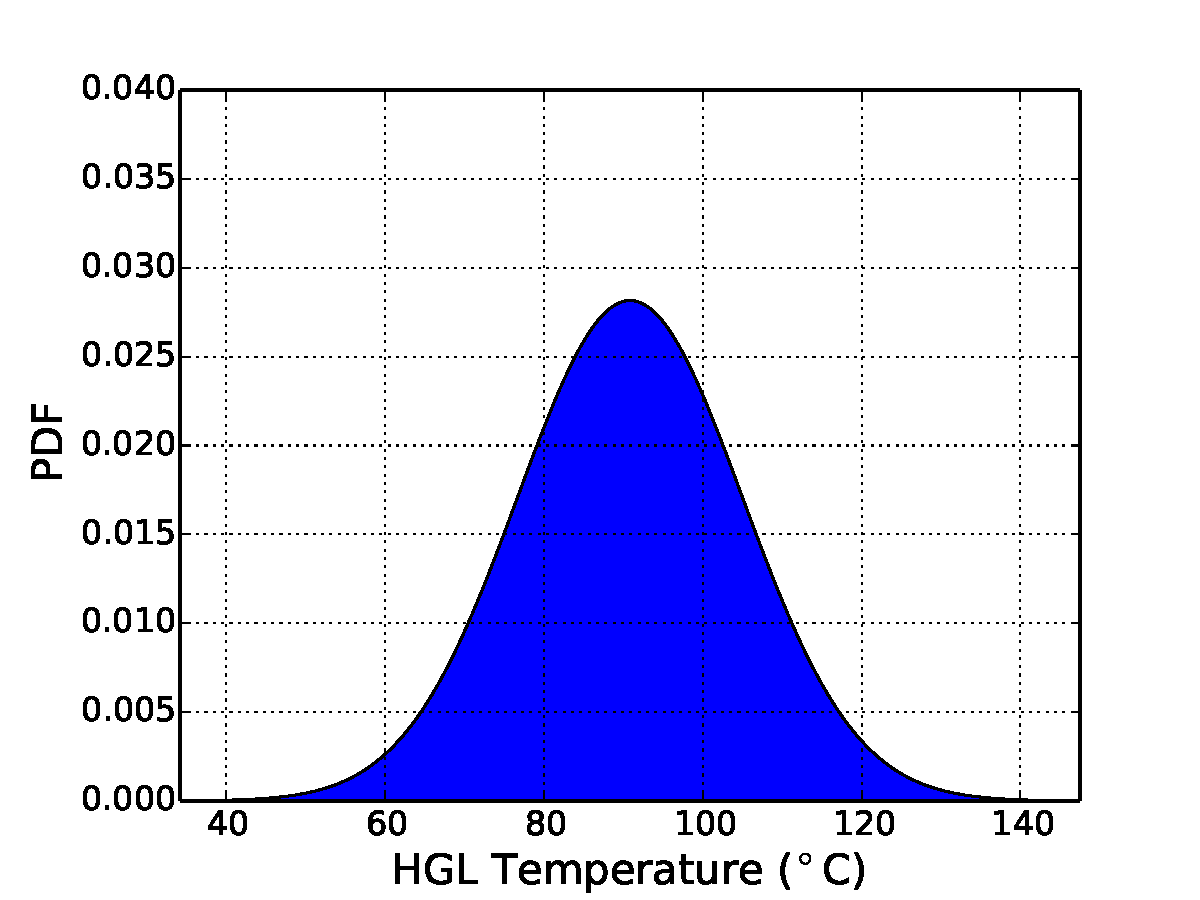
\includegraphics[width=2.6in]{Figures/output_PDF_1_model}
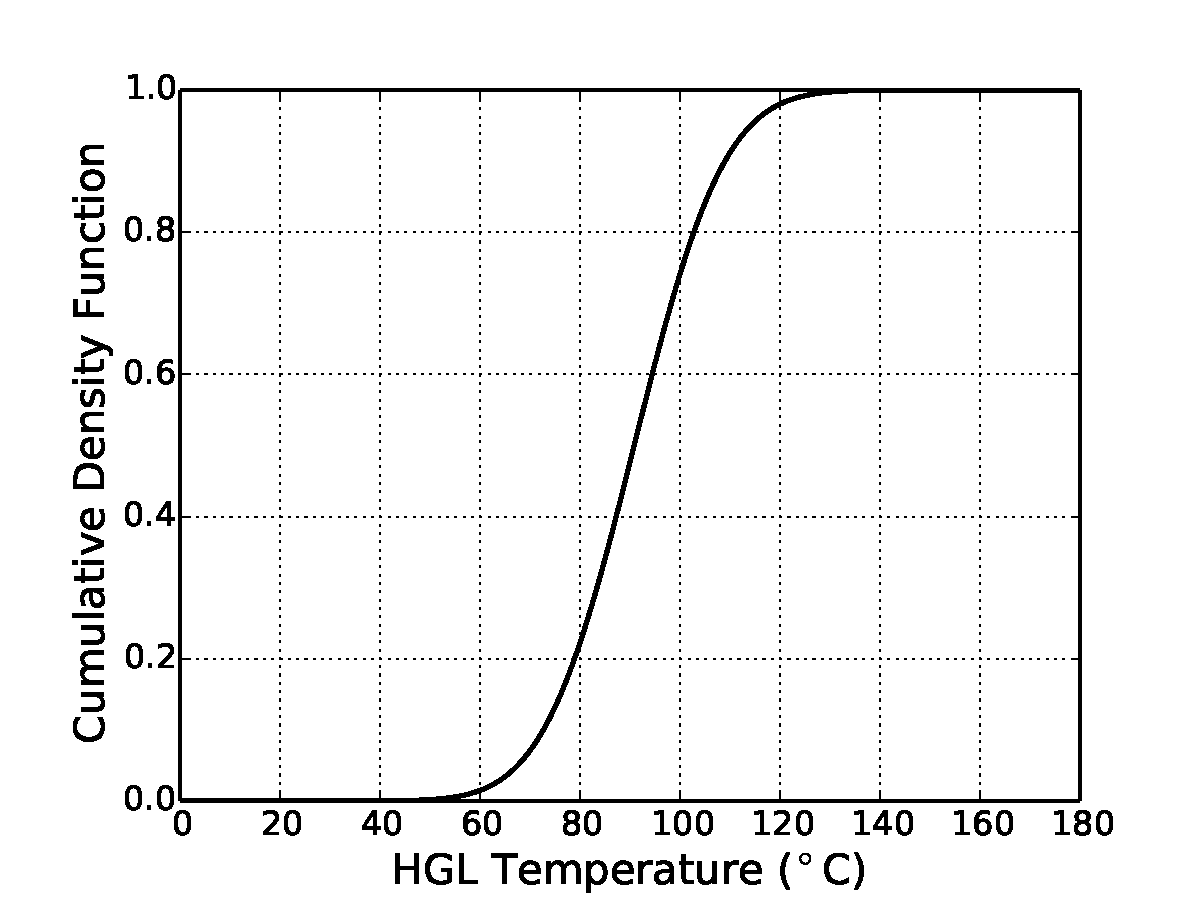
\includegraphics[width=2.6in]{Figures/output_CDF_1_model}
\caption{PDF and CDF of output HGL temperature distribution}
\label{fig:case_1_output_distributions}
\end{figure}

For Case 1, the probability of exceeding the critical HGL temperature of 100~$^\circ$C is calculated as XX.

\subsection{Case 2: Input parameter uncertainty}

This case accounts for input parameter uncertainty.

Consider an input parameter uncertainty of $\pm$20~\% for the HRR. This can be represented as a uniform distribution with a lower and upper bound of 400~kW and 600~kW, respectively. If more information was known about the input parameter, then another distribution could be considered, such as a normal or gamma distribution. A PDF and CDF of the input HRR distribution is shown in Fig.~\ref{fig:case_2_input_distributions}.
\begin{figure}[!ht]
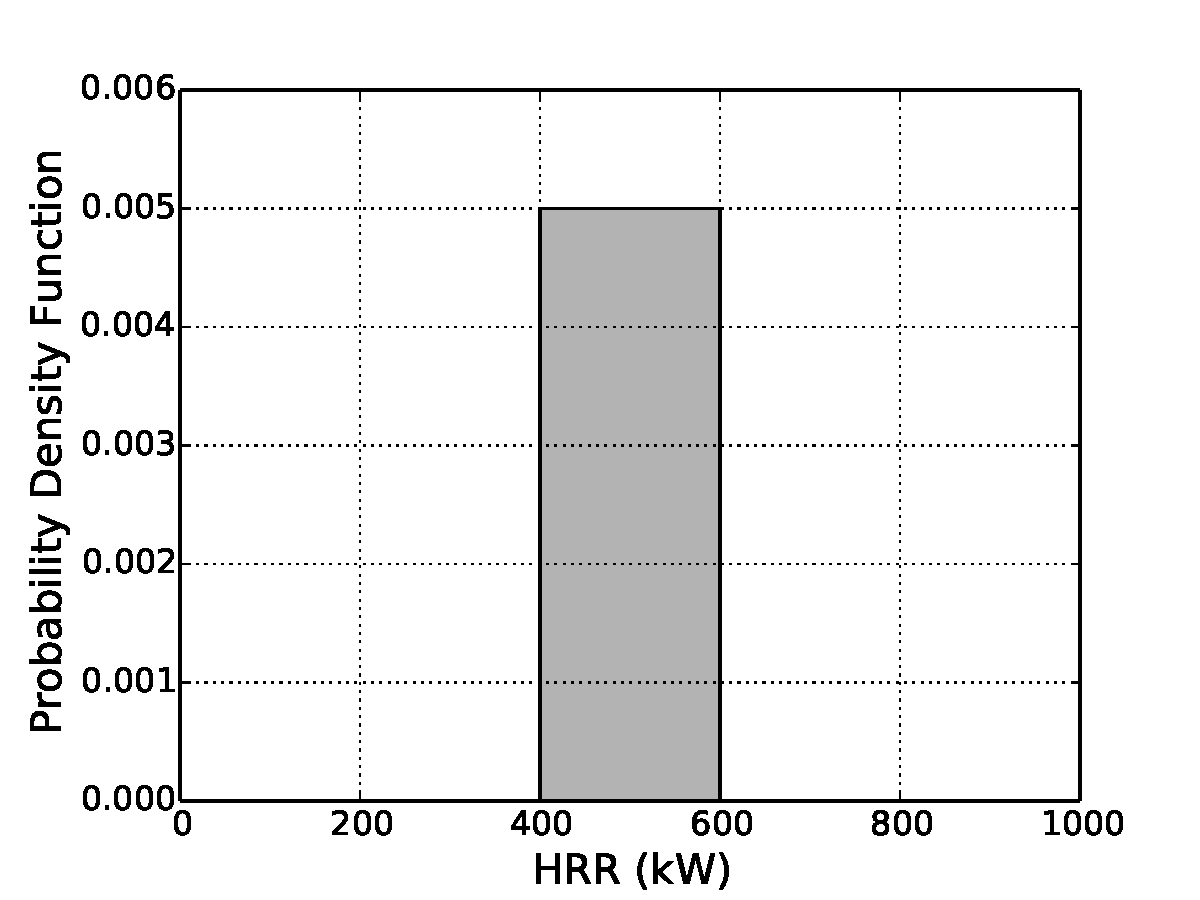
\includegraphics[width=2.6in]{Figures/input_PDF}
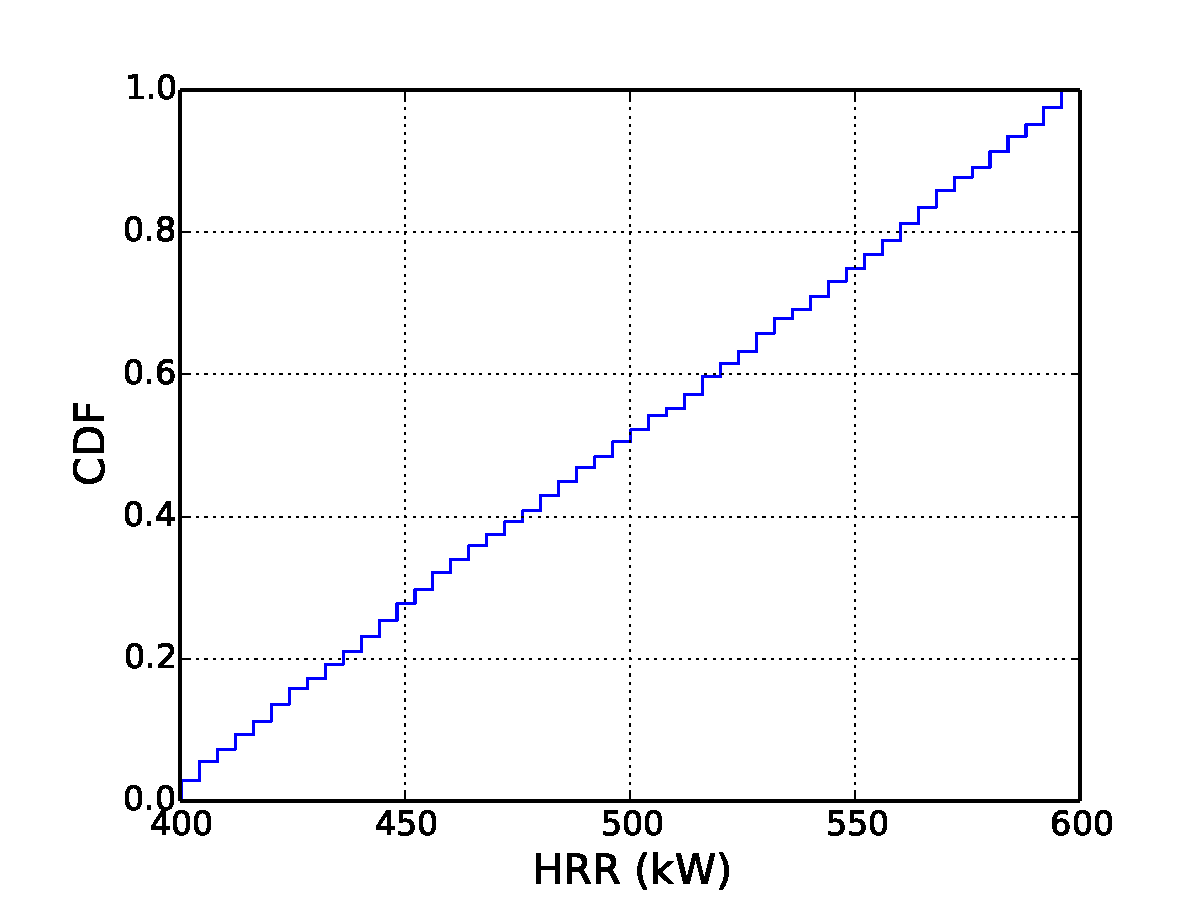
\includegraphics[width=2.6in]{Figures/input_CDF}
\caption{PDF and CDF of input HRR distribution}
\label{fig:case_2_input_distributions}
\end{figure}

The results of Case 2 are shown in Fig.~\ref{fig:case_2_output_distributions}

\begin{figure}[!ht]
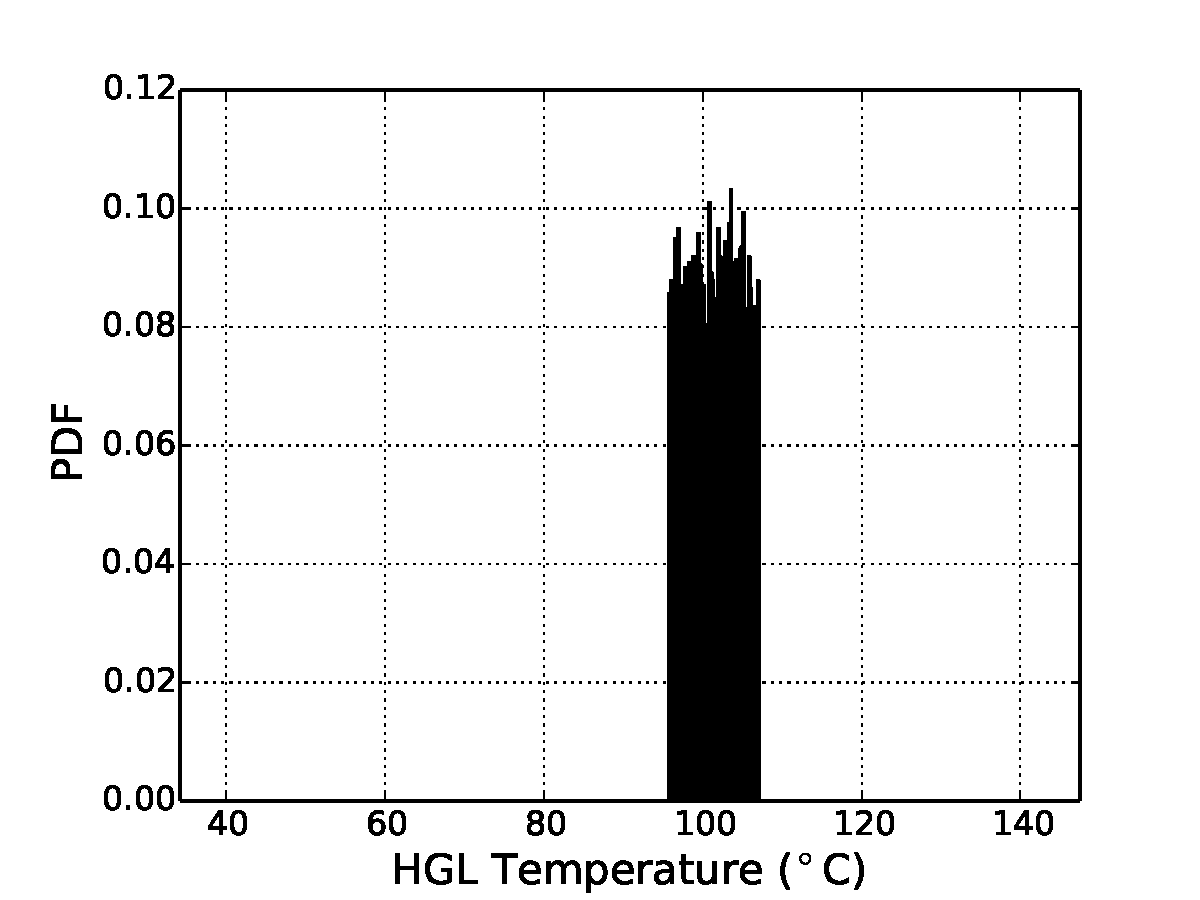
\includegraphics[width=2.6in]{Figures/output_PDF_2_input}
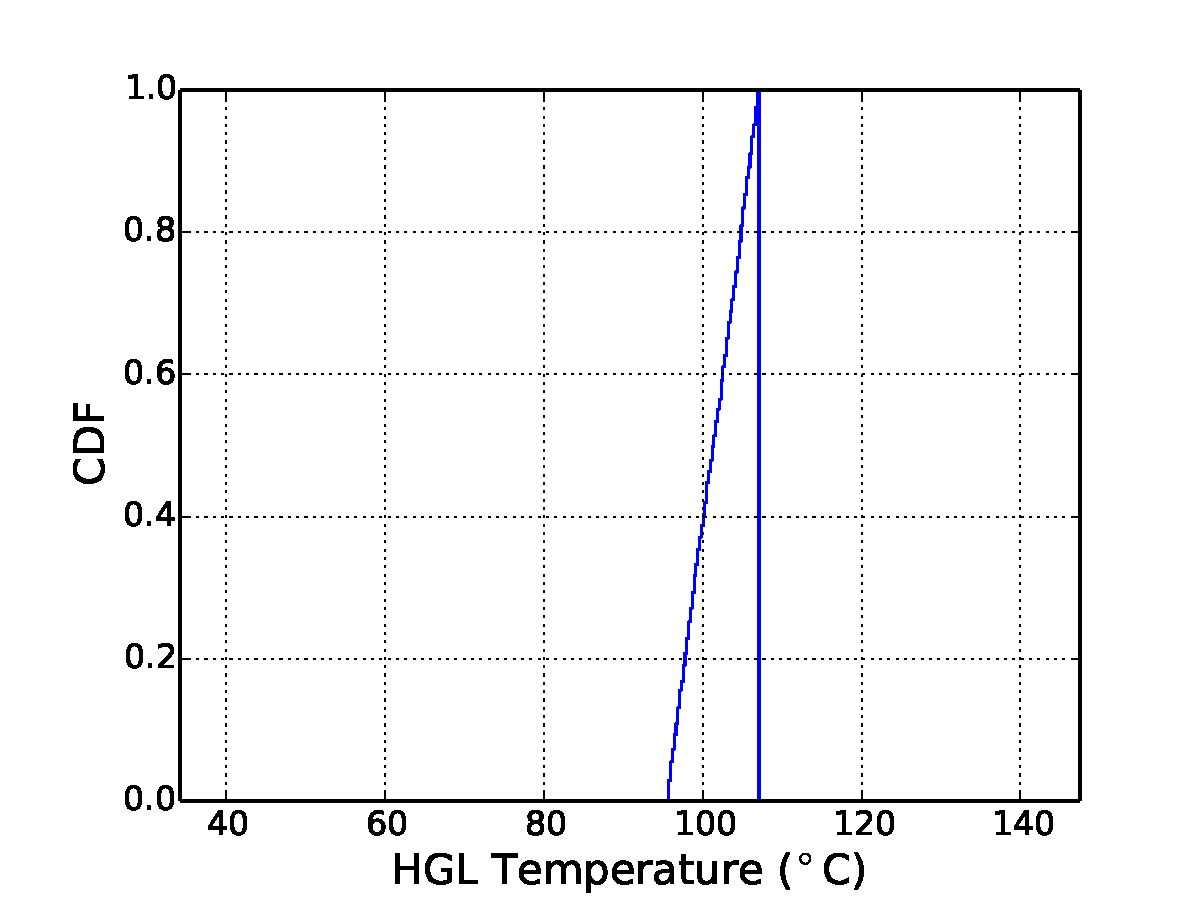
\includegraphics[width=2.6in]{Figures/output_CDF_2_input}
\caption{PDF and CDF of output HGL temperature distribution}
\label{fig:case_2_output_distributions}
\end{figure}

For Case 2, the probability of exceeding the critical HGL temperature of 100~$^\circ$C is calculated as XX.

\subsection{Case 3: Combined model and input parameter uncertainty}

This case accounts for both model bias/uncertainty and input parameter uncertainty.

A PDF and CDF of the input HRR distribution is shown in Fig.~\ref{fig:case_3_input_distributions}.
\begin{figure}[!ht]
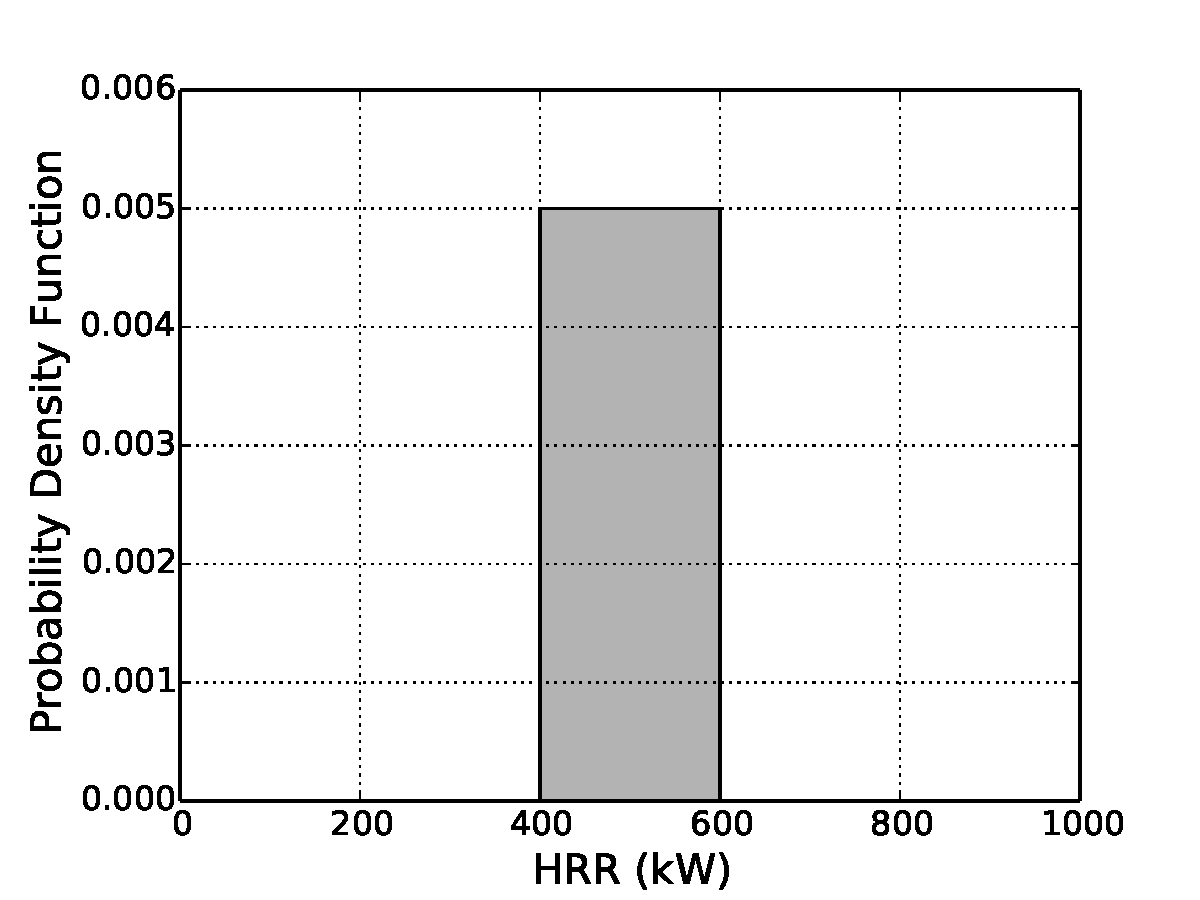
\includegraphics[width=2.6in]{Figures/input_PDF}
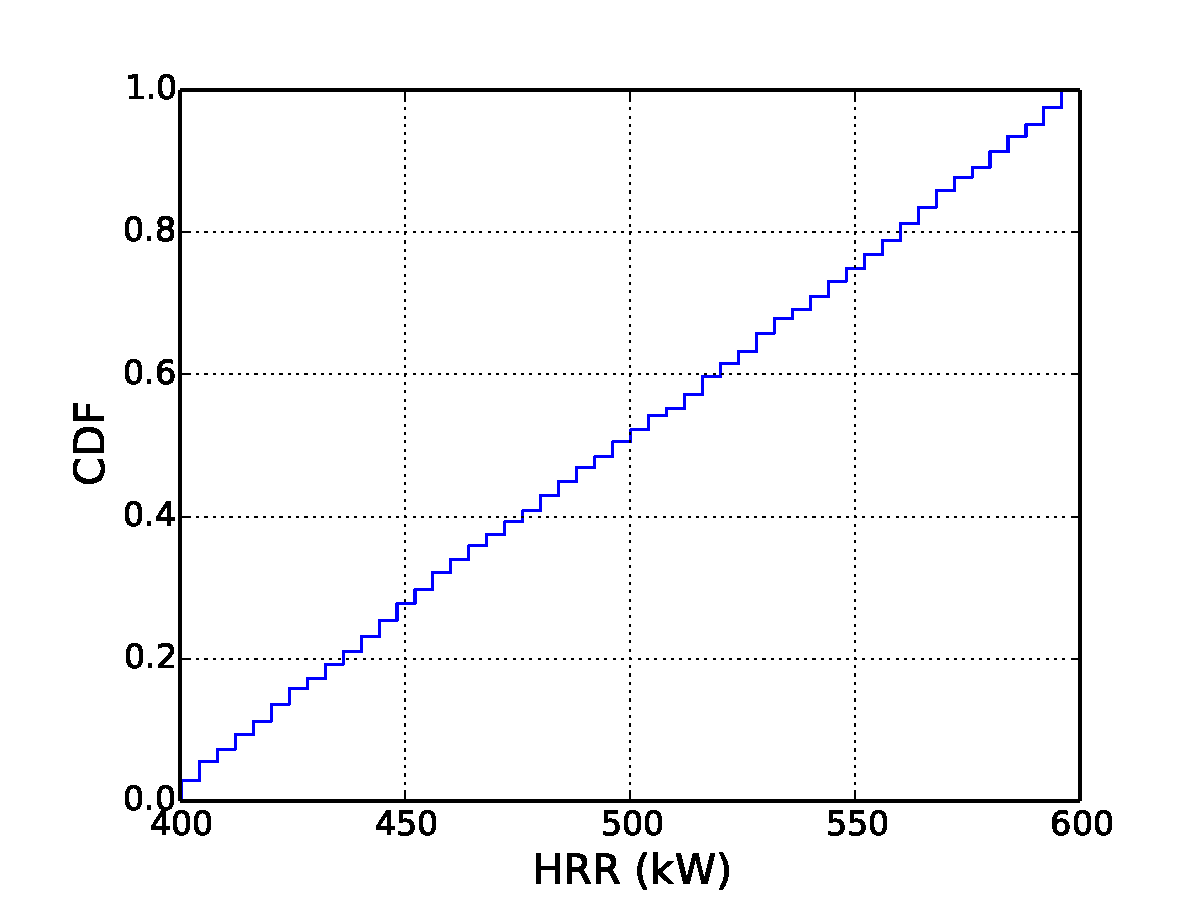
\includegraphics[width=2.6in]{Figures/input_CDF}
\caption{PDF and CDF of input HRR distribution}
\label{fig:case_3_input_distributions}
\end{figure}

The results of Case 2 are shown in Fig.~\ref{fig:case_3_output_distributions}

\begin{figure}[!ht]
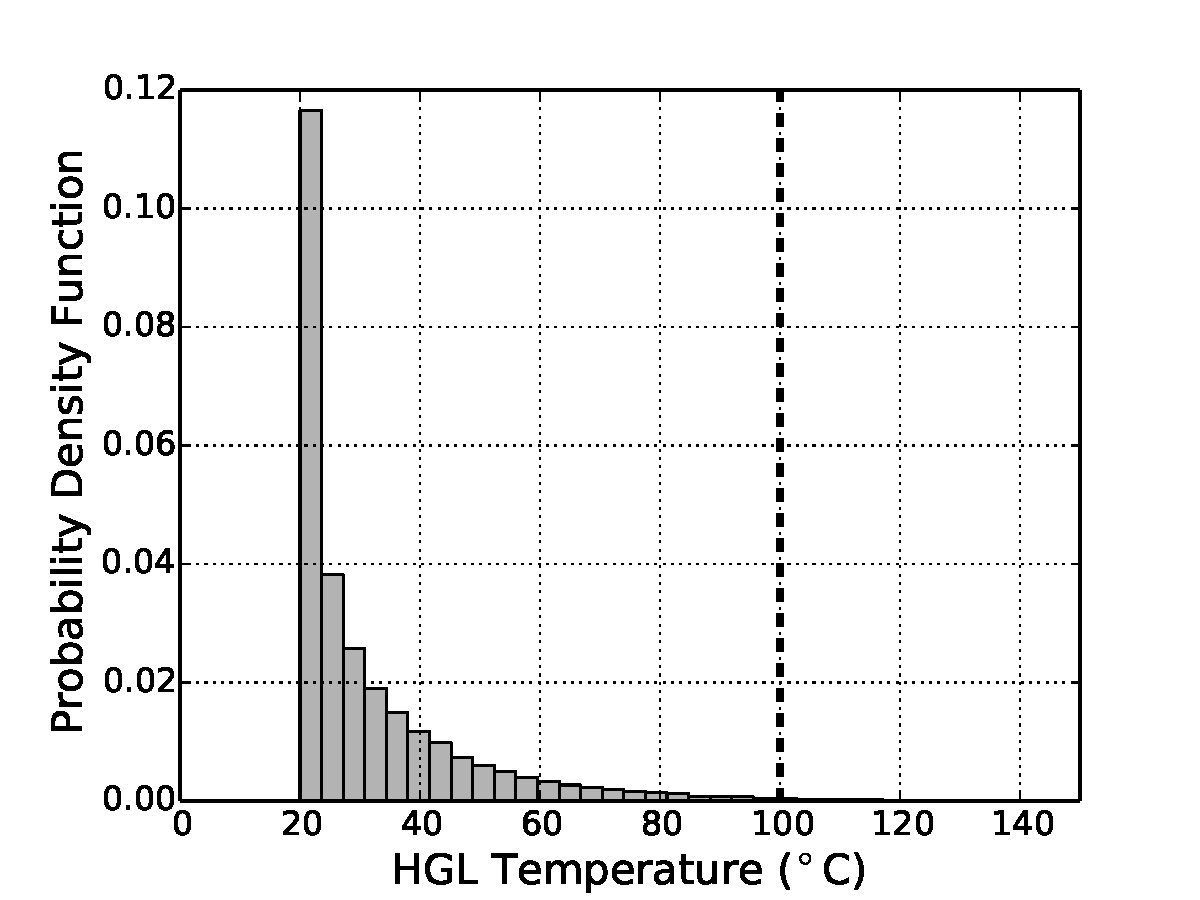
\includegraphics[width=2.6in]{Figures/output_PDF_3_combined}
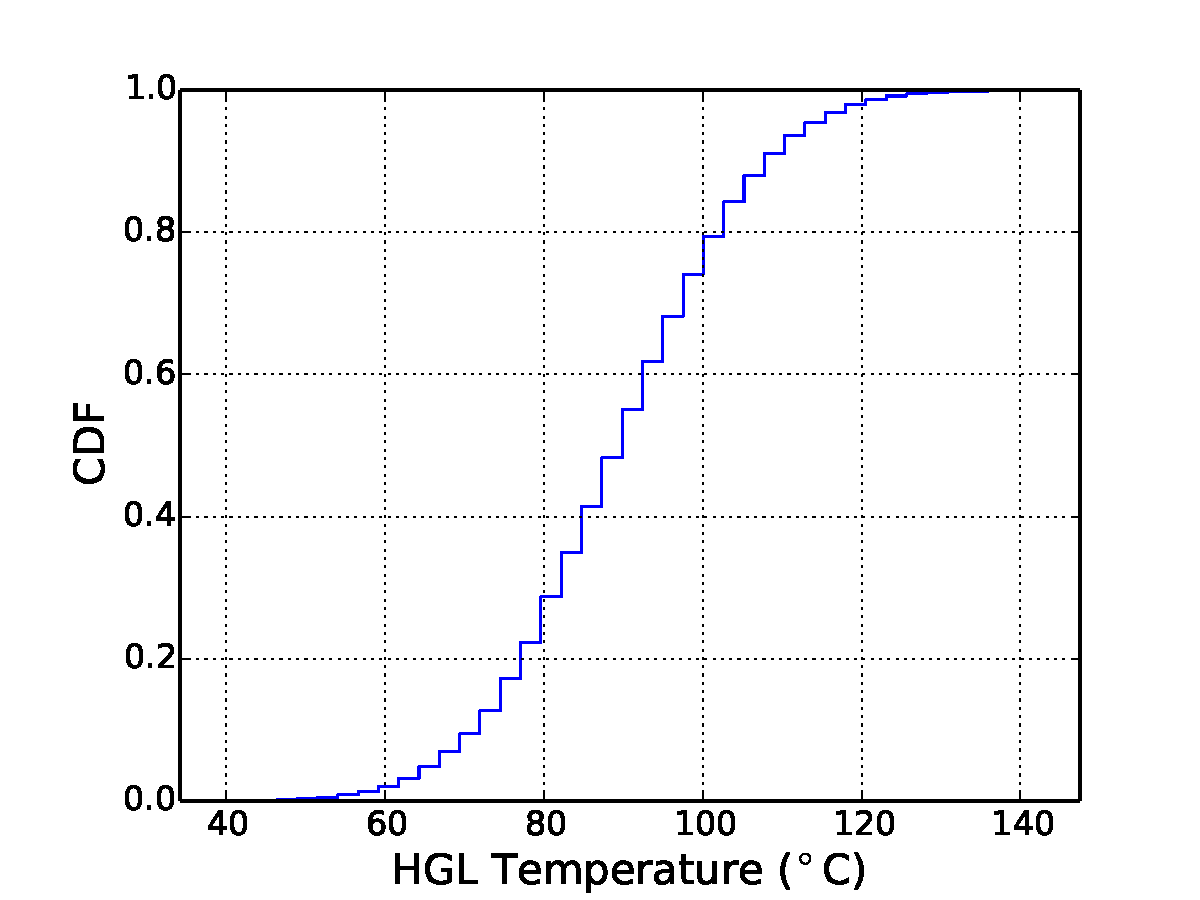
\includegraphics[width=2.6in]{Figures/output_CDF_3_combined}
\caption{PDF and CDF of output HGL temperature distribution}
\label{fig:case_3_output_distributions}
\end{figure}

For Case 3, the probability of exceeding the critical HGL temperature of 100~$^\circ$C is calculated as XX.


\section{Conclusions}
\label{sec:conclusions}


\bibliographystyle{unsrt}
\bibliography{references}

\end{document}